\documentclass[11pt,a4paper]{article}
\usepackage[margin=22mm]{geometry}
\usepackage[T1]{fontenc}
\usepackage{lmodern}
\usepackage{hyperref}
\usepackage{tikz}
\usetikzlibrary{arrows.meta,positioning}
\title{HyMeKo Core on Amaterasu: reproducible container verification}
\date{Created-at: 2026-09-05 13:23 CEST}
\begin{document}
\maketitle
\paragraph{Scope and authorization.}
The user explicitly authorizes Core Dockerization on Amaterasu, prioritizes Core,
and authorizes the subsequent dependency/CI, browser integration and consumer
experiment sequence. This first delivery owns only Core container infrastructure.
Base: audit branch Core 69a5ec947b610a9ccc683d3f8d761d19d30c5b47.
Implementation worktree: D:/hnnwork/amaterasu/core, branch
build/core-amaterasu-2026-09-05. Existing worktrees and services are preserved.
\paragraph{ETA and evidence.}
Approximately 45--90 minutes for the Core container, including 10--25 minutes
for a first remote dependency/image build, 10--25 minutes for cold compilation,
then tests, optional hardware verification and the report. These cold-build times
are estimates, not measurements: the cached Windows suite's 18.91 seconds is not
a Linux cold-build baseline. Inspect logs and resource use at least every minute.
No consumer experiment starts before the Core environment is verified.
\paragraph{Measured update, 2026-09-05 14:03 CEST.}
The initial empty-target CPU container completed in 82.24 seconds, including
compilation, tests and lint. The initial 10--25 minute compilation estimate was
too conservative; budget 1--2 minutes for the final clean-revision CPU run.
An isolated GPU control identified the missing EGL runtime: adding libegl1 to
the otherwise unchanged image enabled the NVIDIA Vulkan adapter. Include it
with libvulkan1 in the container only, then repeat GPU checks without networking.
\section{Ownership and discovery}
Core owns module compilation, validation, canonical IR/hash, CBOR and tensor
primitives. The existing CLI and public CBOR facade supply smoke/correctness
checks. No new model, parser, serializer or runtime service is introduced.
The separate hymeko/hymeko provider owns contract tools; its existing Python
container is reused independently, never vendored into Core.
The Core has no Dockerfile or Docker ignore file. Its only current workflow
checks symbols/duplication and Clippy with incomplete dependency access.
There is one Git dependency in Cargo.lock: parser
e28a205147c48273980e63aa3338ca286974a6ed. The original workspace parent has a
Windows-specific vendor override; it is deliberately excluded from the image.
\section{Affected files and interfaces}
New files: .dockerignore, tools/ci/Dockerfile, tools/ci/core.sh,
docs/core-container.md, this four-file plan bundle, the dated Core report and
reports/core-amaterasu evidence files. Extend .gitattributes only if exact new
artifact bytes or executable shell line endings require it. Existing CI may be
wired to the verified entry point in the subsequent CI phase, after its runner
and authentication are concrete. Protected Core files touched: empty list.
Cargo dependencies, lockfile, fixtures, IR/wire layout and public APIs do not change.
The new container entry point composes existing Cargo commands; invalid actions
must fail. A Rust SDK/dependency image can later support the consumer experiment.
\section{Container and authentication design}
Use the official Rust 1.97.1 Bookworm image, pinned to the verified linux/amd64
manifest digest. Resolve registry metadata and build on Amaterasu itself.
Use a dedicated BuildKit builder with at most 6 CPUs and 16 GiB total memory,
with swap disabled; do not reconfigure the existing ARM builder or services.
Fetch dependencies with Cargo --locked and ephemeral BuildKit SSH/known-host
mounts. Verify the parser host key against the already trusted workstation key;
do not disable host verification or copy private keys into image layers.
The local read-only probe found no parser host-key entry on Amaterasu; resolve
this in the task-owned build environment, not the user's global SSH configuration.
If remote identity lacks repository access, prepare the exact build and continue
independent work while identifying a scoped existing authentication mechanism.
Subsequent compilation and tests run offline, and the final verification container
also runs with Docker networking disabled. Image contains its own writable
source copy because existing hash tests write ignored CSVs in the crate directory.
\section{Verification and resource budgets}
Start with shell syntax/argument checks, pinned toolchain identity, Cargo metadata
and dependency identity audit. Then run the existing Core CLI on the minimal
fixture, canonical CBOR roundtrip/fault tests, the full Core release suite,
workspace formatting and warning-denying Clippy. Run the existing CBOR Criterion
target in smoke mode; this is workload execution evidence, not a timing claim.
Do not explicitly prebuild ir\_depth\_probe: it enables an otherwise skipped
quadratic-memory deep-hierarchy diagnostic. Classify ignored tests by name.
GPU verification is separate and conditional on a real NVIDIA adapter exposed
to the container; never label CPU Vulkan fallback as GPU verification.
Keep all processes under the 16 GiB cgroup cap; retain cgroup memory peak and
wall time, plus exit/OOM states. Container memory includes page cache and is not
identical to process RSS. Cold builds are not benchmark comparisons.
Perform a final build/run from an exact clean Git revision or Git source archive,
recording archive hash, source revision, Docker image digest/ID, toolchain,
dependency versions, commands and test summaries. No laptop target/vendor cache
may serve as the decisive reproduction. Baseline Core source and lock remain exact.
\section{Risks and rollback}
Risks: private Git authentication/name resolution, registry availability,
Linux feature/native-library differences, costly first compilation, GPU runtime
availability, and pre-existing test assumptions. Diagnose the smallest failing
command before changing infrastructure. Protected product fixes require a
separate concrete approval if uncovered; independent infrastructure work continues.
Rollback only this task's named feature commits, images, builder and remote
workspace after checking ownership. Never prune Docker globally, stop existing
services, or publish/merge/tag as a side effect. Local thematic commits are
authorized by the continuing original task. The report records exact scope and
remaining dependency/CI, browser and consumer stages.
\section{Dataflow}
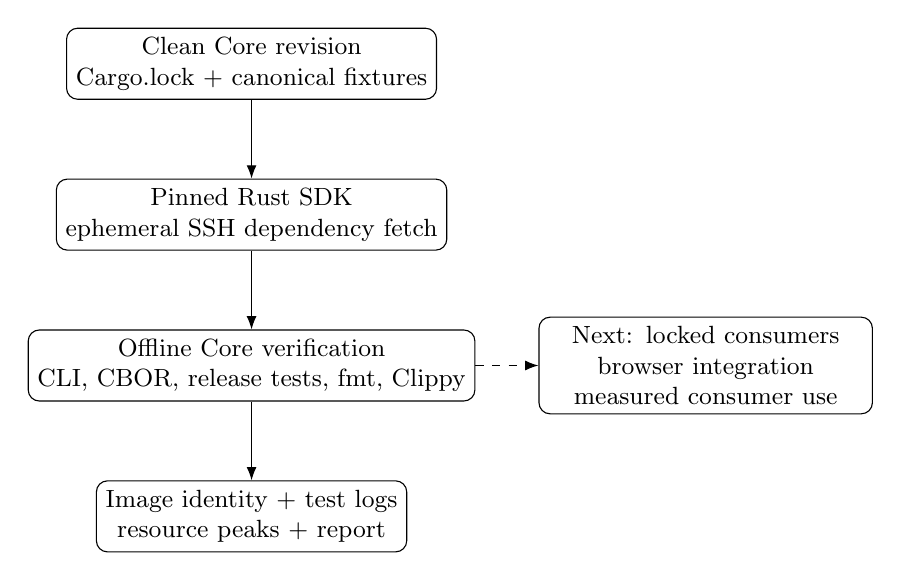
\begin{tikzpicture}[node distance=10mm, every node/.style={draw,rounded corners,align=center,font=\small}, >={Latex}]
\node (source) {Clean Core revision\\Cargo.lock + canonical fixtures};
\node (sdk) [below=of source] {Pinned Rust SDK\\ephemeral SSH dependency fetch};
\node (verify) [below=of sdk] {Offline Core verification\\CLI, CBOR, release tests, fmt, Clippy};
\node (evidence) [below=of verify] {Image identity + test logs\\resource peaks + report};
\node (consumer) [right=8mm of verify,text width=40mm] {Next: locked consumers\\browser integration\\measured consumer use};
\draw[->] (source)--(sdk);
\draw[->] (sdk)--(verify);
\draw[->] (verify)--(evidence);
\draw[->,dashed] (verify)--(consumer);
\end{tikzpicture}

\end{document}
